%%%%%%%%%%%%%%%%%%%%%%%%%%%%%%%%%%%%%%%%%%%%%%%%%%%%%%%%%%%%%%%%%%%%%%
% Overleaf (WriteLaTeX) Example: Molecular Chemistry Presentation
%
% Source: http://www.overleaf.com
%
% In these slides we show how Overleaf can be used with standard 
% chemistry packages to easily create professional presentations.
% 
% Feel free to distribute this example, but please keep the referral
% to overleaf.com
% 
%%%%%%%%%%%%%%%%%%%%%%%%%%%%%%%%%%%%%%%%%%%%%%%%%%%%%%%%%%%%%%%%%%%%%%

\documentclass{beamer}

\mode<presentation>
{
  \usetheme{Madrid}       % or try default, Darmstadt, Warsaw, ...
  \usecolortheme{default} % or try albatross, beaver, crane, ...
  \usefonttheme{default}    % or try default, structurebold, ...
  \setbeamertemplate{navigation symbols}{}
  \setbeamertemplate{caption}[numbered]
} 

\usepackage[english]{babel}
\usepackage[utf8x]{inputenc}
\usepackage{chemfig}
\usepackage[version=3]{mhchem}

\usepackage{hyperref}
  \hypersetup{colorlinks=true}
  \hypersetup{urlcolor=blue}
  \hypersetup{linkcolor = .}
\usepackage{xcolor}
\usepackage{siunitx}
  \sisetup{separate-uncertainty = true}
\usepackage{physics}
\usepackage[font=small,labelfont=bf]{caption}
\usepackage{subcaption}
\usepackage[en-GB]{datetime2}
\usepackage{overpic}
\usepackage{feynmp}
\DeclareGraphicsRule{*}{mps}{*}{}

\usepackage{scalerel}
\newcommand{\mylbrace}[2]{\vspace{#2pt}\hspace{6pt}\scaleleftright[\dimexpr5pt+#1\dimexpr0.06pt]{\lbrace}{\rule[\dimexpr2pt-#1\dimexpr0.5pt]{-4pt}{#1pt}}{.}}
\newcommand{\myrbrace}[2]{\vspace{#2pt}\scaleleftright[\dimexpr5pt+#1\dimexpr0.06pt]{.}{\rule[\dimexpr2pt-#1\dimexpr0.5pt]{-4pt}{#1pt}}{\rbrace}\hspace{6pt}}

% Here's where the presentation starts, with the info for the title slide
\title[BESIII Oxford]{BESIII Oxford Group Meeting}
\author{Martin Tat}
\institute{Oxford LHCb}
\date{17th February 2022}

\titlegraphic{
\includegraphics[width = 4cm, height = 2.8cm]{lhcb.jpg}\hspace{1cm}~%
              
\includegraphics[width = 4cm, height = 2.8cm]{bes3.jpg}}

\begin{document}

\begin{frame}
  \titlepage
\end{frame}

% These three lines create an automatically generated table of contents.
\begin{frame}{Outline}
  \tableofcontents
\end{frame}

\section{\texorpdfstring{$K_L\pi\pi$}{KLpipi} partially reconstructed tag}

\begin{frame}{$K_L\pi\pi$ partially reconstructed tag}
  \begin{itemize}
    \setlength\itemsep{1.0em}
    \item{Previously: Non-sensible Kalman kinematic fits}
    \item{Cause: A single mass constraint insufficient with missing momentum}
    \item{Solution: Fit whole $D^0\bar{D^0}$ decay tree}
  \end{itemize}
  \begin{figure}
    \centering
    \begin{subfigure}{0.49\textwidth}
      \centering
      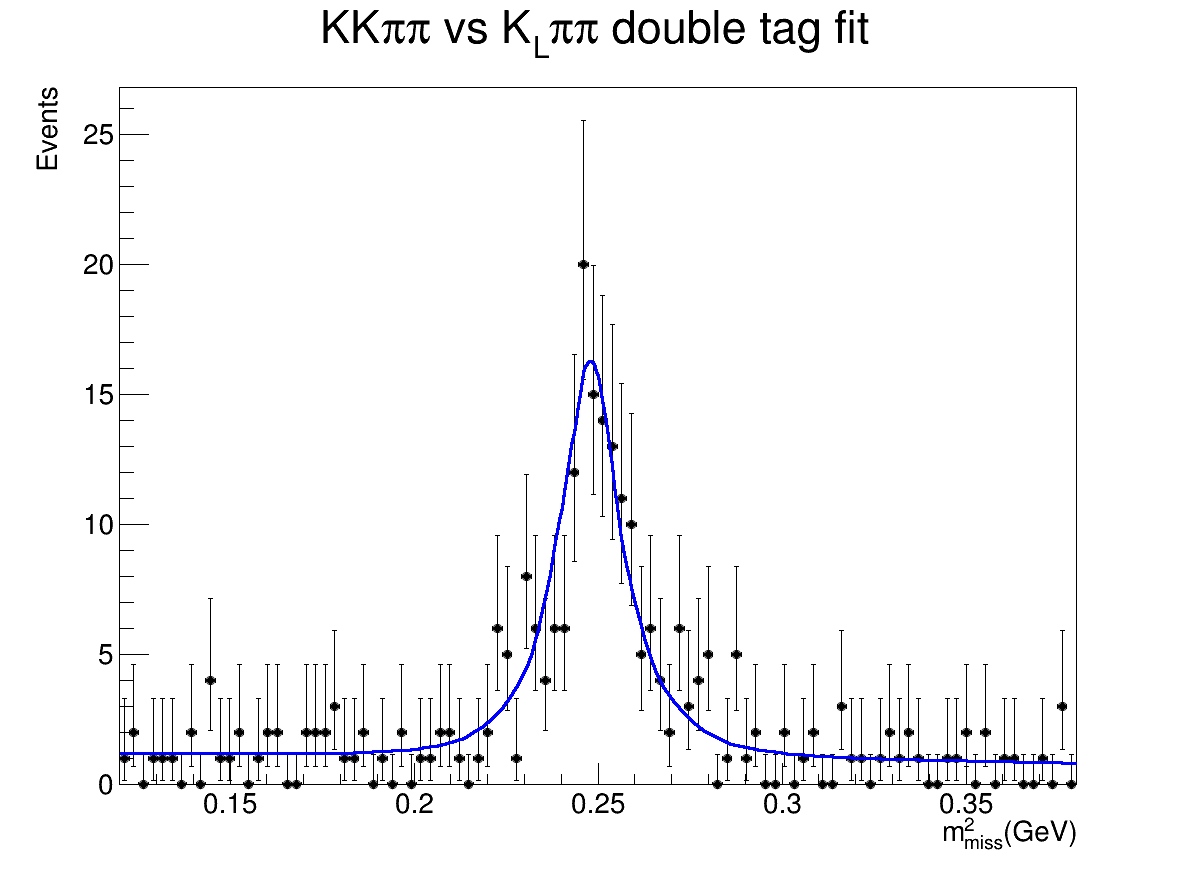
\includegraphics[width=\textwidth]{Plots/KLpipi_Inclusive_DoubleTagYield.png}
      \caption{Inclusive}
    \end{subfigure}%
    \begin{subfigure}{0.49\textwidth}
      \centering
      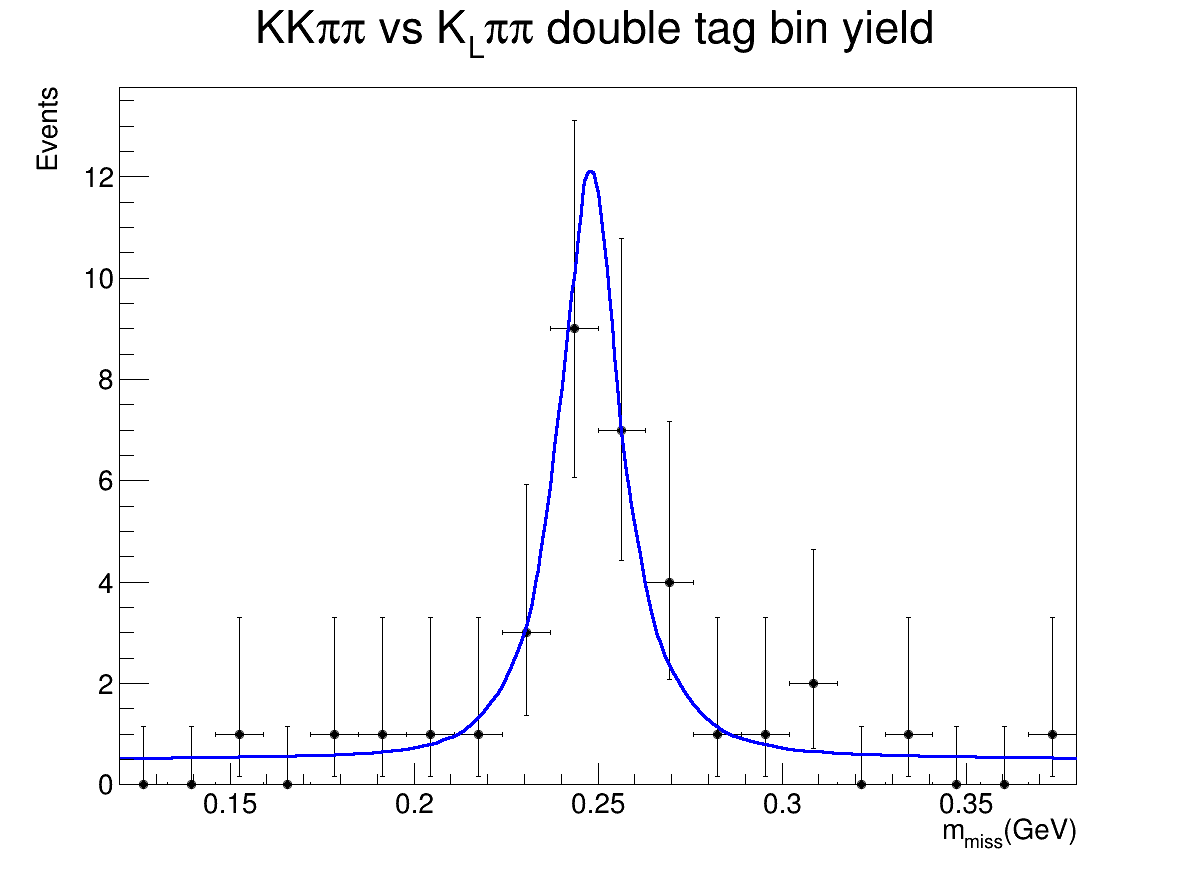
\includegraphics[width=\textwidth]{Plots/KLpipi_1_DoubleTagYield.png}
      \caption{$KK\pi\pi$ bin $1$+$2$, $K_S\pi\pi$ bin $6$+$7$+$8$}
    \end{subfigure}
    \caption{Signal shape from MC, background is 1st order polynomial}
  \end{figure}
\end{frame}

\section{Partially reconstructed \texorpdfstring{$KK\pi\pi$}{KKpipi} vs \texorpdfstring{$K_S\pi\pi$}{KSpipi}}

\begin{frame}{Partially reconstructed $KK\pi\pi$ vs $K_S\pi\pi$}
  \begin{itemize}
    \setlength\itemsep{1.0em}
    \item{Reconstruct $K_S\pi\pi$ first}
    \item{Require exactly 3 charged tracks on the other side ($K\pi\pi$)}
    \item{Problem: Large, non-peaking background under signal!}
  \end{itemize}
  \begin{figure}
    \centering
    \begin{subfigure}{0.49\textwidth}
      \centering
      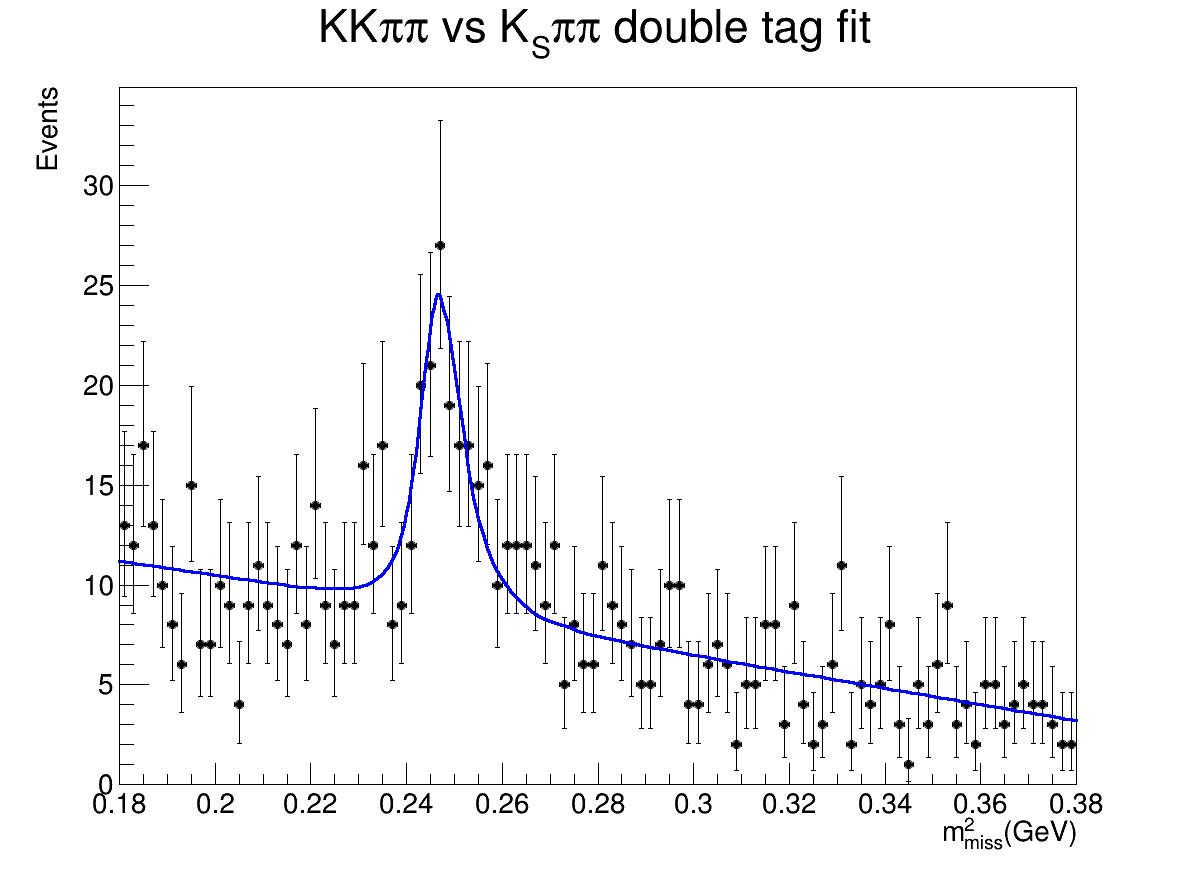
\includegraphics[width=\textwidth]{Plots/KSpipiPartRecoNoPi0Veto_Inclusive_DoubleTagYield.png}
      \caption{Inclusive}
    \end{subfigure}%
    \begin{subfigure}{0.49\textwidth}
      \centering
      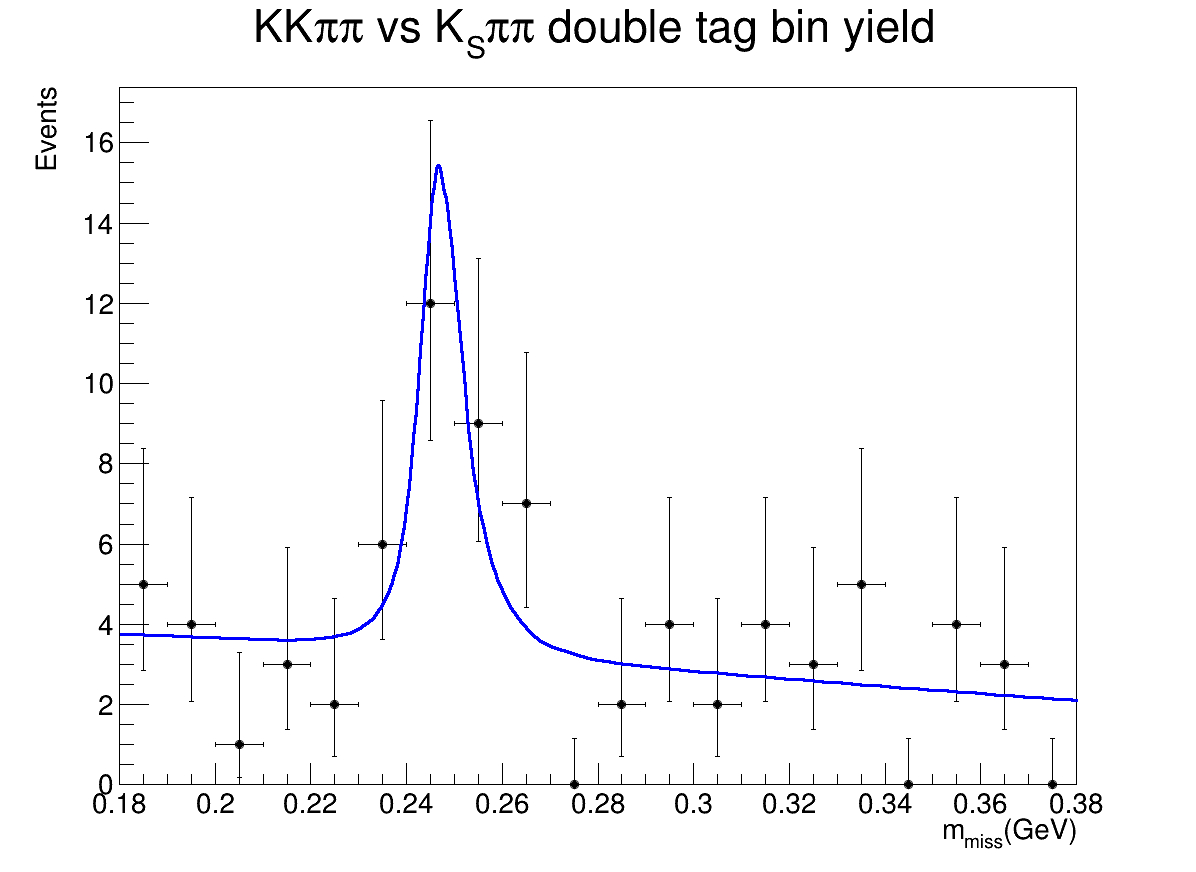
\includegraphics[width=\textwidth]{Plots/KSpipiPartRecoNoPi0Veto_1_DoubleTagYield.png}
      \caption{$KK\pi\pi$ bin $1$+$2$, $K_S\pi\pi$ bin $6$+$7$+$8$}
    \end{subfigure}
    \caption{Signal shape from MC, background is 1st order polynomial}
  \end{figure}
\end{frame}

\begin{frame}{Partially reconstructed $KK\pi\pi$ vs $K_S\pi\pi$}
  \begin{itemize}
    \setlength\itemsep{1.0em}
    \item{Background mostly from $K\pi\pi\pi\pi^0$}
    \item{Veto any events with $\pi^0$}
  \end{itemize}
  \begin{figure}
    \centering
    \begin{subfigure}{0.49\textwidth}
      \centering
      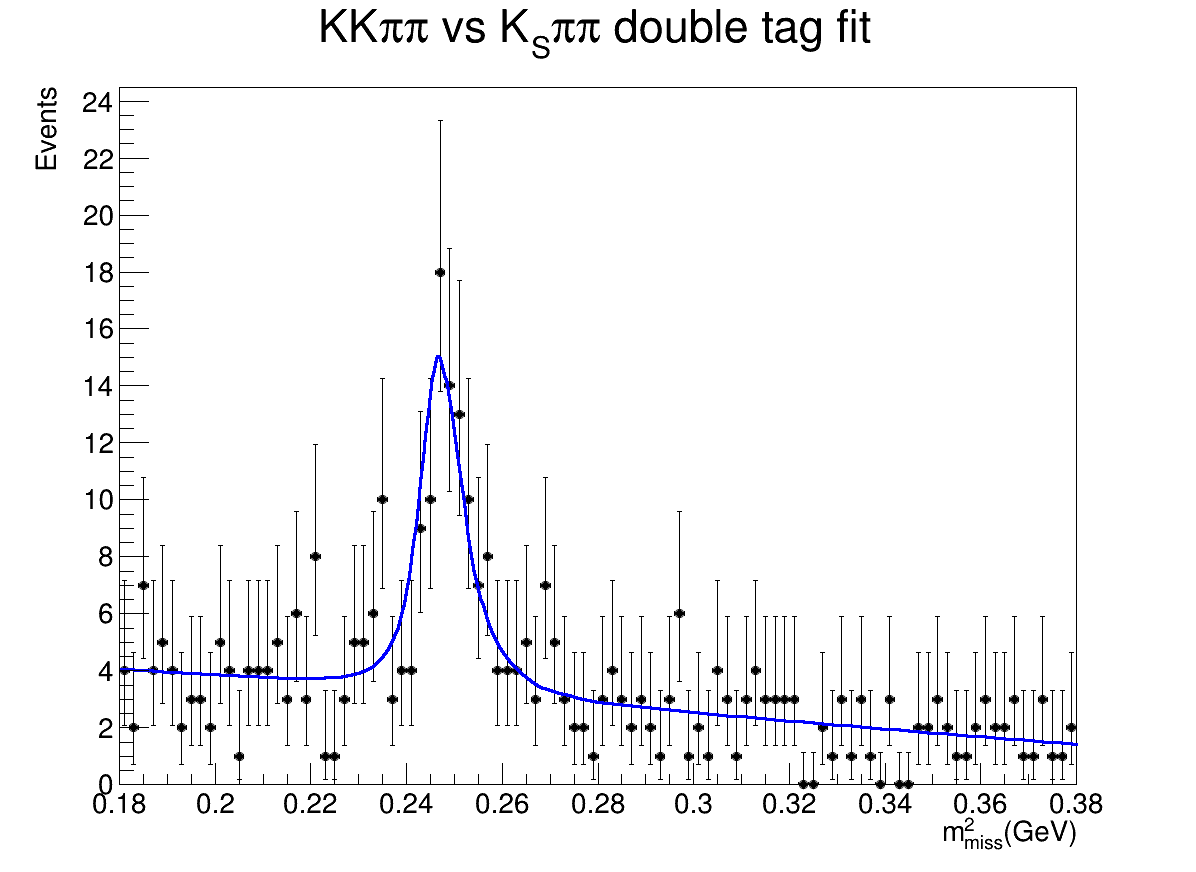
\includegraphics[width=\textwidth]{Plots/KSpipiPartReco_Inclusive_DoubleTagYield.png}
      \caption{Inclusive}
    \end{subfigure}%
    \begin{subfigure}{0.49\textwidth}
      \centering
      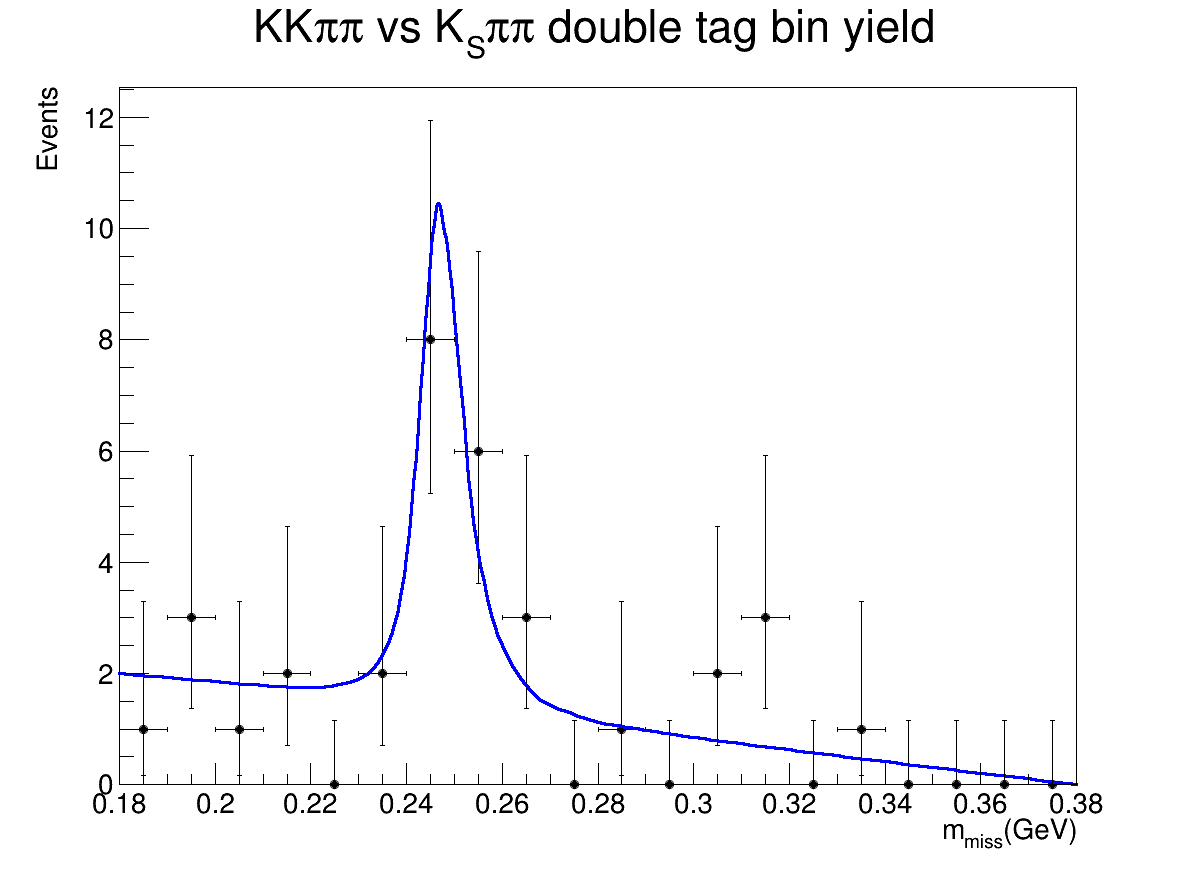
\includegraphics[width=\textwidth]{Plots/KSpipiPartReco_1_DoubleTagYield.png}
      \caption{$KK\pi\pi$ bin $1$+$2$, $K_S\pi\pi$ bin $6$+$7$+$8$}
    \end{subfigure}
    \caption{Signal shape from MC, background is 1st order polynomial}
  \end{figure}
\end{frame}

\begin{frame}{Summary of $K^0\pi\pi$ yields and efficiencies}
  \centering
  \def\arraystretch{1.2}%
  \begin{tabular}{l|c|c}
    Mode                                     & Inclusive yield & Double tag efficiency \\
    \hline
    $K_L\pi\pi$ (fully reconstructed)        & $158.7$         & $6.93 \pm 0.04$ \\
    $K_S\pi\pi$ (fully reconstructed)        & $67.2$          & $6.63 \pm 0.04$ \\
    $K_S\pi\pi$ (partially reconstructed)    & $85.9$          & $6.50 \pm 0.03$ \\
    $K_S\pi\pi$ (part reco, no $\pi^0$ veto) & $116.0$         & $9.04 \pm 0.04$ \\
    \hline
  \end{tabular}
\end{frame}

\section{Quantum correlation correction of \texorpdfstring{$K_SKK$}{KSKK} background}

\begin{frame}{Quantum correlation correction of $K_SKK$ background}
  \begin{itemize}
    \setlength\itemsep{1.0em}
    \item{$K_SKK\to KK\pi\pi$ is a background in all tags}
    \item{Must account for QC in CP tags}
    \item{$K_SKK$ $F_+ = 0.524\pm0.018$ from $F_+ = \frac{1}{2} + \sum_i\sqrt{K_iK_{-i}}c_i$}
    \begin{itemize}
      \item{Similar constributions from $K_S\phi$ (odd) and $K_Sa_0(980)^0$ (even)}
    \end{itemize}
    \item{Strategy:}
    \begin{enumerate}
      \item{Generate signal MC of $K_SKK$ vs CP tag}
      \item{Account for relative bin efficiency}
      \item{Calculate ``effective'' $F_+$}
    \end{enumerate}
    \item{Results:}
    \begin{itemize}
      \item{$KK$ tag (even): $F_+ = 0.726\pm0.030$}
      \item{$K_S\pi^0$ tag (odd): $F_+ = 0.840\pm0.034$}
    \end{itemize}
  \end{itemize}
\end{frame}

\begin{frame}{Quantum correlation correction of $K_SKK$ background}
  \begin{itemize}
    \setlength\itemsep{1.0em}
    \item{To first order $K_SKK$ background is independent of tag mode}
    \item{Use $KK$ and $K_S\pi^0$ shape and ``effective'' $F_+$ for CP even and odd tags, respectively}
  \end{itemize}
  \begin{figure}
    \centering
    \begin{subfigure}{0.49\textwidth}
      \centering
      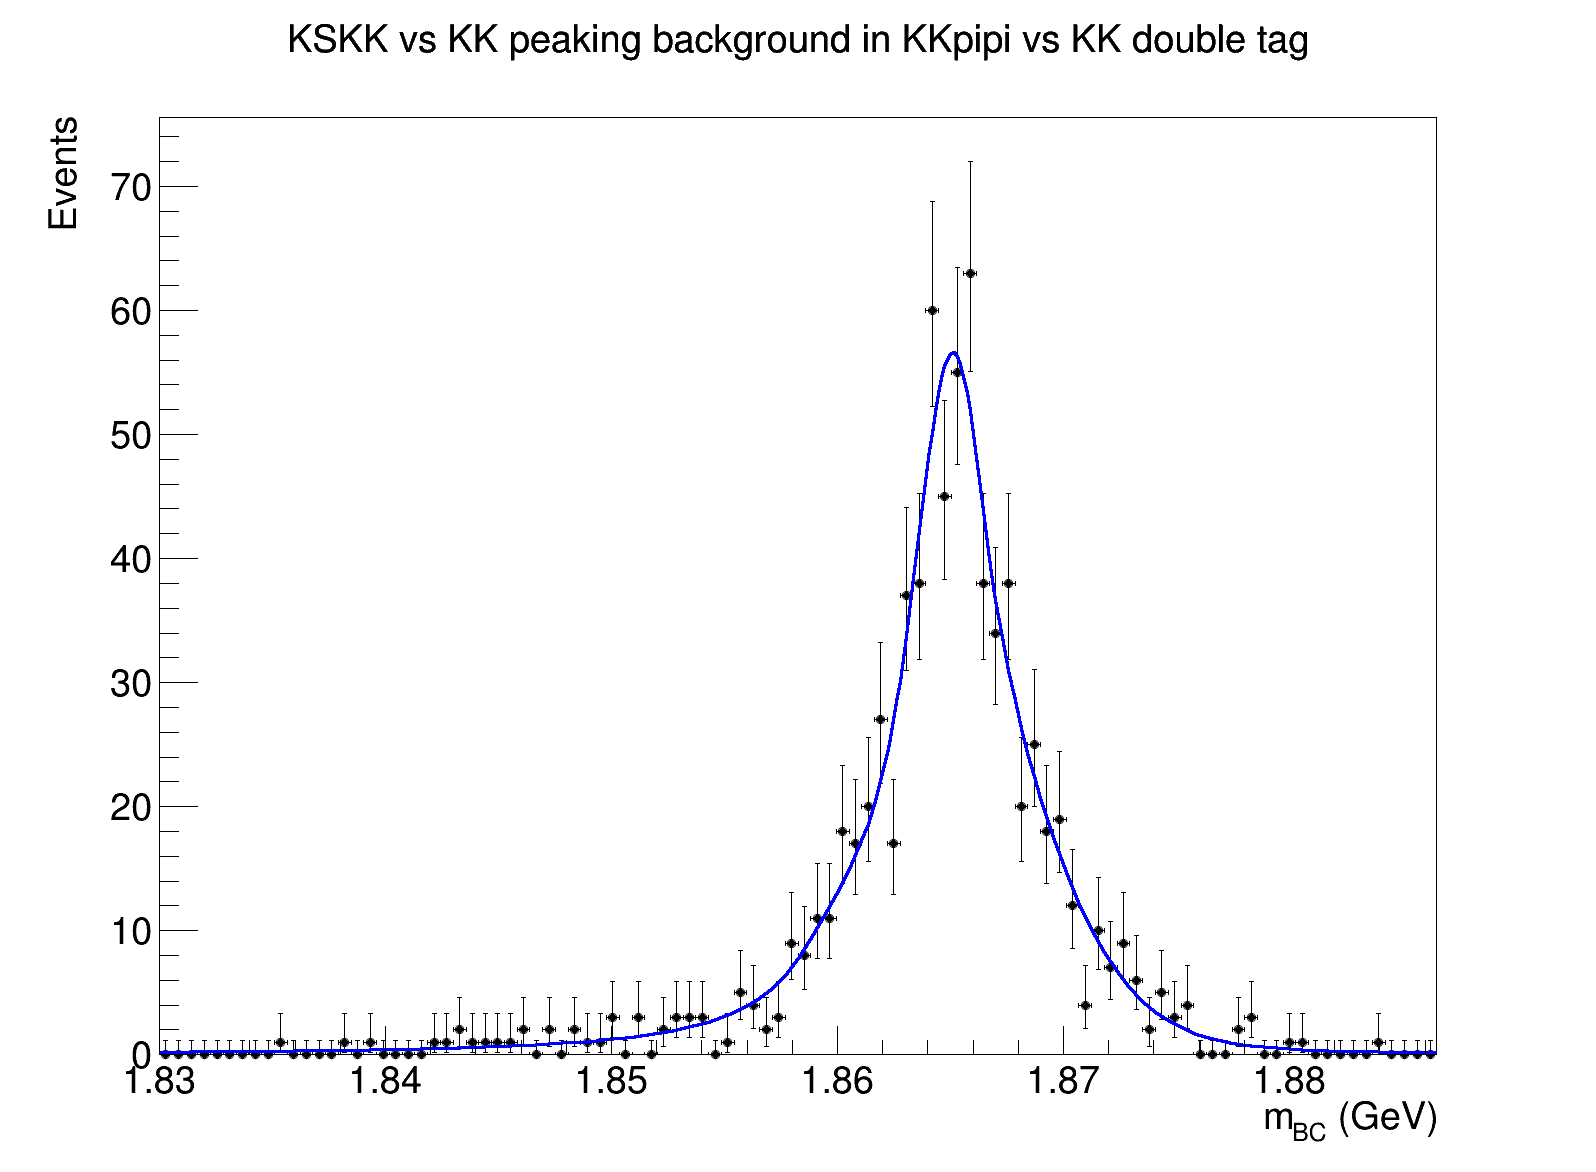
\includegraphics[width=\textwidth]{Plots/KSKK_to_KKpipi_vs_KK_DoubleTag_FitPlot.png}
      \caption{$KK$ tag}
    \end{subfigure}%
    \begin{subfigure}{0.49\textwidth}
      \centering
      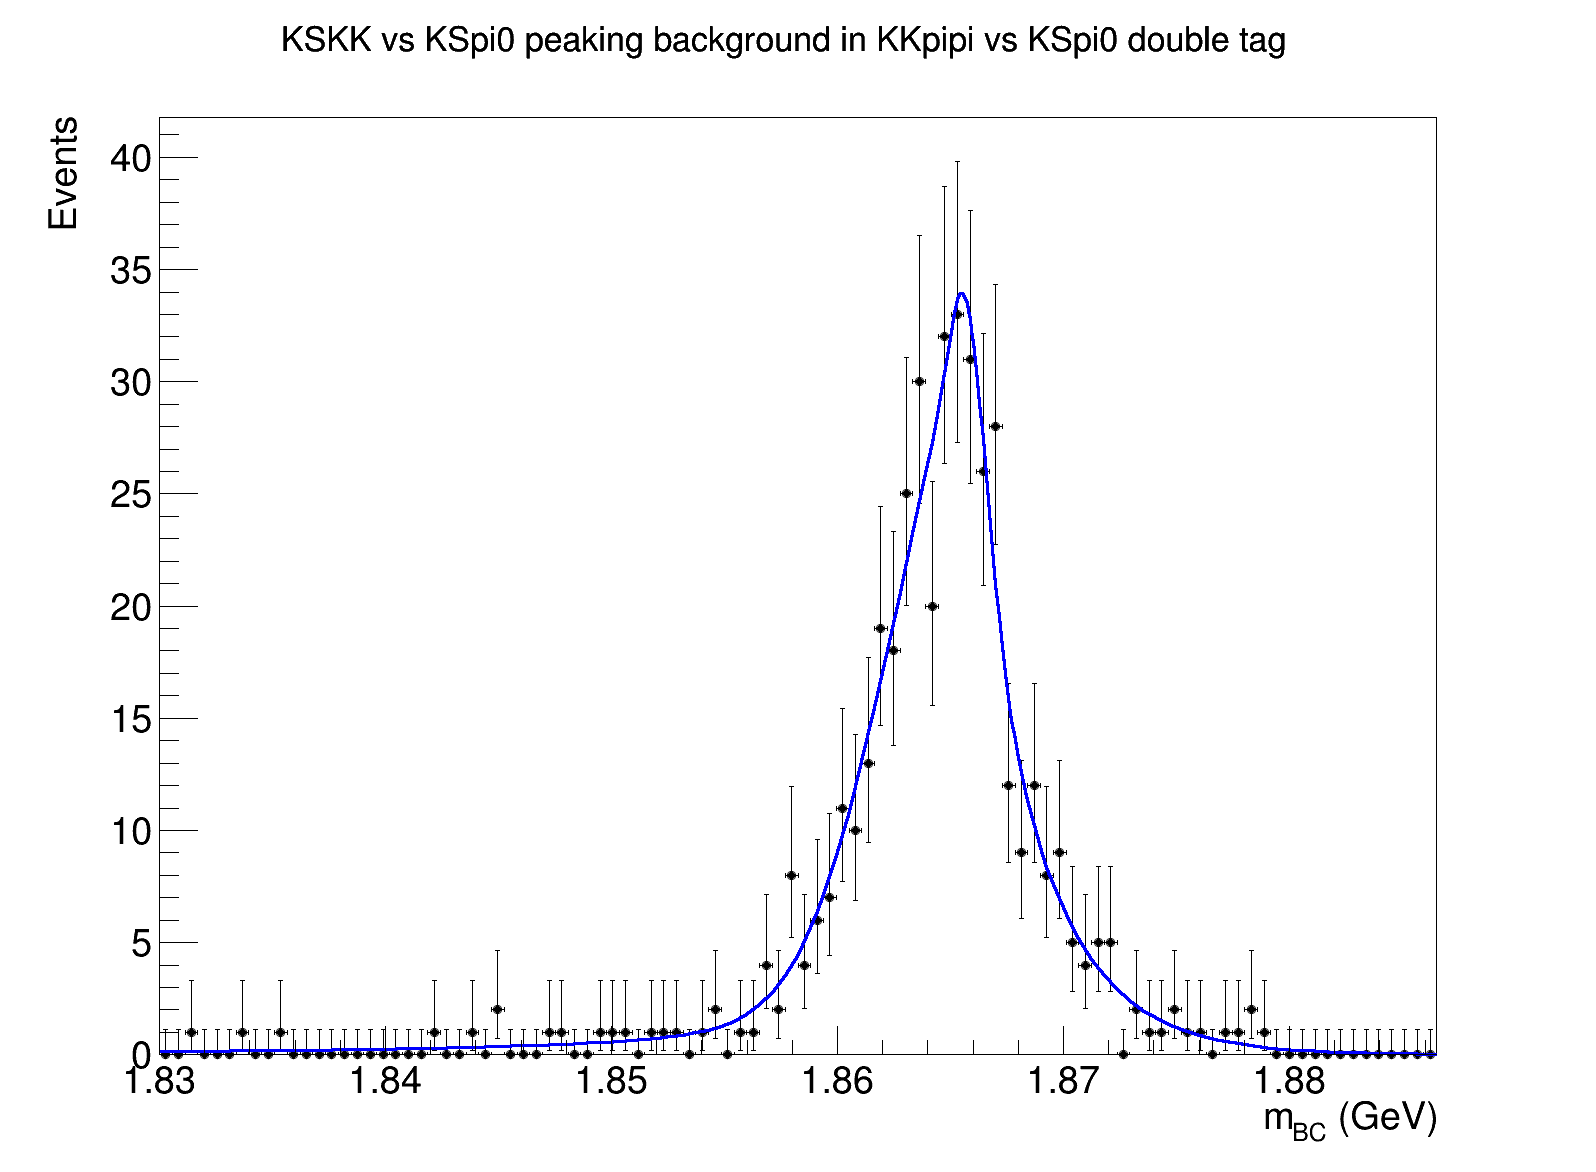
\includegraphics[width=\textwidth]{Plots/KSKK_to_KKpipi_vs_KSpi0_DoubleTag_FitPlot.png}
      \caption{$K_S\pi^0$ tag}
    \end{subfigure}
    \caption{$K_SKK$ background shape for CP even and odd tags}
  \end{figure}
\end{frame}

\begin{frame}{Conclusion and next steps}
  \begin{itemize}
    \setlength\itemsep{1.5em}
    \item{Conclusion:}
    \begin{itemize}
    \setlength\itemsep{0.5em}
      \item{$K_L\pi\pi$ tag works with sensible yields}
      \item{Partially reconstructed $KK\pi\pi$ vs $K_S\pi\pi$ increases sensitivity to $s_i$}
      \item{Quantum correlation of $K_SKK\to KK\pi\pi$ background is accounted for with ``effective'' $F_+$ in CP tags}
    \end{itemize}
    \item{Next steps:}
    \begin{enumerate}
    \setlength\itemsep{0.5em}
      \item{Finalize treatment of peaking backgrounds in all CP tags}
      \item{Combine all single and double tag yields, after efficiency corrections, to fit $KK\pi\pi$ $F_+$}
      \item{Binned analysis of $K_S\pi\pi$ and $K_L\pi\pi$ in $F_+$ measurement}
    \end{enumerate}
  \end{itemize}
\end{frame}

\end{document}
